\documentclass[aspectratio=43,11pt]{beamer}
\usepackage{amsmath,amssymb,booktabs,xcolor,soul}
\usetheme{default}
\usecolortheme{default}
\setbeamertemplate{navigation symbols}{}
\setbeamertemplate{footline}[frame number]
\definecolor{aggiemaroon}{RGB}{80,0,0}
\setbeamercolor{structure}{fg=aggiemaroon}
\setbeamertemplate{itemize items}[circle]
\usepackage{tikz}
\usetikzlibrary{arrows.meta,positioning}
\usepackage{pgfplots}
\pgfplotsset{compat=1.18}
\newcommand{\E}{\mathbb{E}}
\newcommand{\Prob}{\mathbb{P}}
\newcommand{\dd}{\mathcal D}
\title{Decision and Risk Analysis}
\subtitle{Lecture 9: \textbf{Bayesian Simple Normal Regression}}
\author{}
\date{\color{aggiemaroon}{DAEN 427 / ISEN 427 / ISEN 627 - Fall 2026\\
      \textbf{Alexander Abuabara}}}
\titlegraphic{\vfill 
\includegraphics[height=1.2cm]{TAMU_logo.png}}

\begin{document}
\begin{frame}
\titlepage
\end{frame}

\begin{frame}{Learning goals}
\begin{enumerate}
\item Identify when Normal regression is appropriate.
\item Interpret coefficients, residual variation, and priors.
\item Use posterior simulations for inference and prediction.
\item Apply predictive uncertainty to risk-based decisions.
\item Assess model limitations before acting.
\end{enumerate}
\end{frame}

\begin{frame}{The business question: tomorrow bike demand}
Capital Bikeshare wants enough bikes available to serve customers, without paying for excessive spare capacity.
\begin{itemize}
\item Outcome $Y$: number of rides on a day.
\item Predictor $X$: temperature (the data use \texttt{temp\_feel}).
\item Modeling question: how does typical ridership vary with temperature?
\item Decision question: how much capacity should we prepare given a forecast of $75^\circ$F?
\end{itemize}
\end{frame}

\begin{frame}[fragile]{R: fit the model}
\footnotesize
\begin{verbatim}
library(tidyverse)
library(bayesrules)
library(rstanarm)
data(bikes)

glimpse(bikes)

summary(bikes[, c("rides", "temp_feel")])

nrow(bikes)

lm(rides ~ temp_feel,
   data = bikes)
\end{verbatim}
\par\medskip\textbf{Crucial/pivotal:} estimating the mean is not the same as forecasting one unpredictable day.
\end{frame}

\begin{frame}{Model choice comes before computation}
\small
\begin{enumerate}
\item What kind of response is $Y$?\\ \footnotesize{Rides are counts, but daily values can be large.}
\item Is a Poisson model reasonable?\\\footnotesize{A Poisson imposes $\operatorname{Var}(Y)=\E(Y)$;\\historical bike demand is/can be much more variable.}
\begin{itemize}
\item \footnotesize{Bike demand may fluctuate by hundreds of rides because of weather, weekends, holidays, and other factors.}
\item \footnotesize{If the observed variance exceeds the mean, we call this overdispersion.}
\end{itemize}
\item A Normal model may be a useful approximation to the broad, roughly bell-shaped variation.
\begin{itemize}
\item \footnotesize{Temperature explains some, but not all, of that variation.}
\item \footnotesize{Start with Normal regression, then check:}
\begin{itemize}
\item \footnotesize{Whether the residuals are approximately Normal.}
\item \footnotesize{Whether variability changes with temperature.}
\item \footnotesize{Whether predictions are realistic, especially for unusually demands.}
\end{itemize}
\end{itemize}
\end{enumerate}
\end{frame}

\begin{frame}{From one overall mean to a temperature-specific mean}
\textbf{Modeling decision:} start with Normal regression; later test fit and check whether predictions behave sensibly (especially in tails).

\[Y_i\mid\mu,\sigma\sim N(\mu,\sigma^2)\qquad\Longrightarrow\qquad
Y_i\mid\beta_0,\beta_1,\sigma\sim N(\mu_i,\sigma^2)\]
\[\boxed{\mu_i=\beta_0+\beta_1 X_i}\]

\begin{itemize}
\item $\beta_0$: fitted mean at $X=0$\\ \footnotesize{(possibly outside a meaningful range).}
\item $\beta_1$: expected additional rides per one-degree increase.
\item $\sigma$: day-to-day standard deviation \emph{at a fixed temperature}.
\end{itemize}
\par\medskip
\textbf{Example:} $\mu=-2000+100X$ predicts $5000$ rides at $70^\circ$F.
The negative intercept is an extrapolation, not negative actual demand.
\end{frame}

\begin{frame}{Same trend, different risk}
\centering
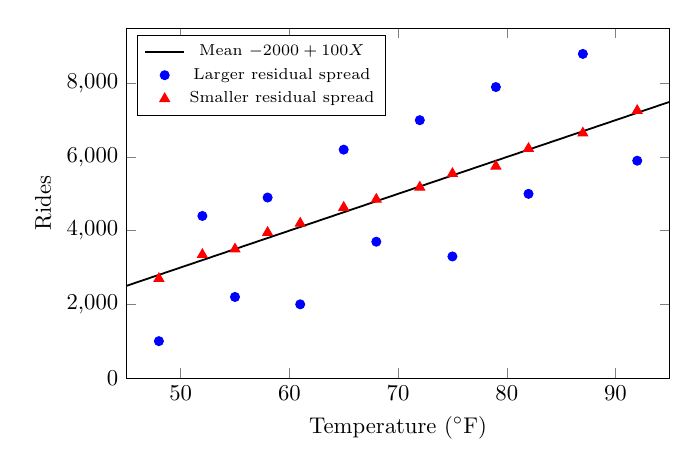
\begin{tikzpicture}[scale=.82]
\begin{axis}[width=10cm,height=7.0cm,xmin=45,xmax=95,ymin=0,ymax=9500,xlabel={Temperature ($^\circ$F)},ylabel={Rides},legend style={font=\scriptsize,at={(.02,.98)},anchor=north west}]
\addplot[thick,black,domain=45:95]{-2000+100*x};\addlegendentry{Mean $-2000+100X$}
\addplot[only marks,mark=*,mark size=2pt,blue] coordinates {(48,1000)(52,4400)(55,2200)(58,4900)(61,2000)(65,6200)(68,3700)(72,7000)(75,3300)(79,7900)(82,5000)(87,8800)(92,5900)};\addlegendentry{Larger residual spread}
\addplot[only marks,mark=triangle*,mark size=2.5pt,red] coordinates {(48,2700)(52,3350)(55,3500)(58,3950)(61,4200)(65,4630)(68,4850)(72,5180)(75,5550)(79,5750)(82,6230)(87,6650)(92,7260)};\addlegendentry{Smaller residual spread}
\end{axis}\end{tikzpicture}
\par\medskip
\scriptsize Synthetic points:
both have the same slope; larger $\sigma$ makes tomorrow demand harder to predict.
\end{frame}

\begin{frame}{What assumptions are we choosing?}
\begin{enumerate}
\item \textbf{Conditional independence:} after accounting for $X$, observations do not depend on each other.
\item \textbf{Linear mean:} $\E(Y_i\mid X_i)=\beta_0+\beta_1 X_i$.
\item \textbf{Normal errors:} departures from the line are approximately Normal.
\item \textbf{Constant spread:} the same $\sigma$ applies at every $X$.
\end{enumerate}
\par\medskip Could weekends, holidays, seasonality, or weather patterns break these assumptions?
Why might a forecast be risky on an unusually hot day?
\end{frame}

\begin{frame}{Bayesian regression = likelihood + priors}
\begin{align*}
Y_i\mid\beta_0,\beta_1,\sigma &\stackrel{ind}{\sim} N(\beta_0+\beta_1X_i,\sigma^2),\\
\beta_0&\sim N(m_0,s_0^2),\\
\beta_1&\sim N(m_1,s_1^2),\\
\sigma&\sim\operatorname{Exp}(\lambda).
\end{align*}
These priors describe plausible parameter values \emph{before} observing the modeled dataset. An Exponential prior keeps $\sigma>0$.
\par\medskip\textbf{Choice:} tune priors to real knowledge; avoid priors implying absurd ridership changes or implausible fluctuations.
\begin{itemize}
\item \footnotesize{Bayesian regression uses the likelihood to describe the data, priors to express initial uncertainty, and the posterior to update our knowledge about regression parameters.}
\item \footnotesize{Important: Priors should be checked against real-world knowledge, ideally using prior predictive simulations before fitting the model.}
\end{itemize}
\end{frame}

\begin{frame}{Centering gives the intercept practical meaning}
Define $X_c=X-70$; then
\[\mu=\beta_{0c}+\beta_1(X-70),\qquad \beta_{0c}=\beta_0+70\beta_1.\]

\begin{itemize}
\item $\beta_{0c}$ means typical rides at $70^\circ$F.
\item $\beta_0$ means a hypothetical average at $0^\circ$F.
\item Both parameterizations imply \emph{the same line} when transformed consistently.
\end{itemize}
\par\medskip
\textbf{Prior intuition:} 5,000 rides at a typical temperature is easier to assess than $-2,000$ at freezing temperatures.
\end{frame}

\begin{frame}{Informed priors}
\[\beta_{0c}\sim N(5000,1000^2),\quad \beta_1\sim N(100,40^2),\quad \sigma\sim\operatorname{Exp}(0.0008).\]

\begin{itemize}
\item Baseline: about 3,000--7,000 rides on a typical day (roughly 95\% prior range).
\item Slope: around 100 additional rides per $1^\circ$F, with appreciable uncertainty.
\item Residual SD: prior mean $1/0.0008=1250$ rides.
\end{itemize}

\par\medskip
\textbf{Prior predictive check:} simulate lines \emph{and whole datasets}. Do these imply believable high-demand days, low-demand days, and uncertainty?
\end{frame}

\begin{frame}{Prior predictive checks prevent poor decisions}
\begin{center}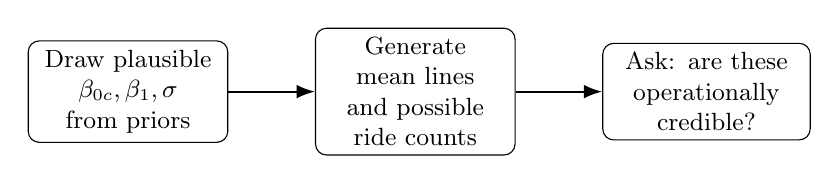
\begin{tikzpicture}[>=Latex,node distance=1.1cm,every node/.style={font=\small}]
\node[draw,rounded corners,text width=2.3cm,align=center] (a) {Draw plausible $\beta_{0c},\beta_1,\sigma$ from priors};
\node[draw,rounded corners,text width=2.3cm,align=center,right=of a] (b) {Generate mean lines and possible ride counts};
\node[draw,rounded corners,text width=2.4cm,align=center,right=of b] (c) {Ask: are these operationally credible?};
\draw[->,thick] (a)--(b);\draw[->,thick](b)--(c);
\end{tikzpicture}\end{center}
A prior can look reasonable for each parameter separately yet produce unbelievable combinations.
\par\medskip\textbf{Action:} revise the prior or the model \emph{before} interpreting posterior probabilities as business risks.
\end{frame}

\begin{frame}{Updating with 500 observed days}
The example uses a sample of 500 days with \texttt{rides} and \texttt{temp\_feel}.
\[p(\beta_0,\beta_1,\sigma\mid\dd)\propto
\underbrace{p(\beta_0,\beta_1,\sigma)}_{\text{prior}}
\underbrace{\prod_{i=1}^{n}p(y_i\mid x_i,\beta_0,\beta_1,\sigma)}_{\text{likelihood}}.\]
The posterior is not a simple familiar distribution.\\
\textbf{MCMC} approximates it using many plausible parameter triples.\\
The draw $(-2200,83,1300)$ describes one possible line and one possible residual spread; it is \emph{not} a separate fitted model selected in isolation.
\end{frame}

\begin{frame}[fragile]{R: fit the model using \texttt{rstanarm}}
\footnotesize
\begin{verbatim}
library(bayesrules)
library(rstanarm)
data(bikes)

bike_model <- stan_glm(
  rides ~ temp_feel,
  data = bikes,
  family = gaussian,
  prior_intercept = normal(5000, 1000),
  prior = normal(100, 40),
  prior_aux = exponential(0.0008),
  chains = 4, iter = 10000, seed = 84735
)
\end{verbatim}
% \scriptsize As in the book, \texttt{rstanarm} \texttt{prior\_intercept} applies to the internally centered predictor.
\end{frame}

\begin{frame}{Check the simulation before trusting it}
\begin{itemize}
\item \textbf{Trace plots:} chains should mix and explore similar parameter regions.
\item \textbf{$\widehat R$ near 1:} evidence of stable between-chain behavior.
\item \textbf{Effective sample size:} enough independent information from simulated draws.
\item \textbf{Also inspect warnings:} divergences and other sampler problems matter.
\end{itemize}
It reports $\widehat R$ values near 1 for its fitted bike model.
\par\medskip\textbf{Risk:} bad computation can create unwarranted confidence, even when the regression equation looks correct.
\end{frame}

\begin{frame}{What the posterior says}
\centering\small
\begin{tabular}{lrr}
\toprule Parameter & Posterior estimate & 80\% credible interval\\\midrule
Intercept $\beta_0$ & $-2194$ & $[-2656,-1732]$\\
Slope $\beta_1$ & $82.2$ & $[75.6,88.8]$\\
Residual SD $\sigma$ & $1281$ & $[1231,1336]$\\\bottomrule
\end{tabular}

\[\widehat\mu(x)\approx -2194.24+82.16x.\]

\begin{itemize}
\item A one-degree increase is associated with about 82 more \emph{expected} rides.
\item Credible intervals summarize uncertainty about parameters, not day-to-day rides.
\item This is association, not proof that changing temperature causes ridership to change.
\end{itemize}
\end{frame}

\begin{frame}{Probability is more actionable than a yes/no claim}
With posterior draws $\beta_1^{(1)},\ldots,\beta_1^{(S)}$,
\[\Prob(\beta_1>0\mid\dd)\approx\frac1S\sum_{s=1}^{S}\mathbf 1\{\beta_1^{(s)}>0\}.\]
In the 20,000 saved draws, all simulated slopes are positive, giving an \emph{estimated} probability of approximately 1.
\par\medskip\textbf{But:} near-certain positive association does \emph{not} imply near-certain daily demand. $\sigma\approx1281$ still leaves large unexplained fluctuation.
\end{frame}

\begin{frame}{Two questions that must not be confused}
At $75^\circ$F, the fitted mean is
\[\widehat\mu(75)=-2194.24+82.16(75)\approx3968.\]
\begin{block}{Question A: average ridership at $75^\circ$F}
How uncertain is the \emph{mean} $\mu(75)$?\\
Only parameter uncertainty matters.
\end{block}
\begin{block}{Question B: ridership tomorrow at $75^\circ$F}
How uncertain is one \emph{future observation} $Y_{\mathrm{new}}$?\\
Parameter uncertainty \emph{plus} residual day-to-day variability matter.
\end{block}
\end{frame}

\begin{frame}{Posterior prediction: one extra simulation step}
For each saved posterior draw $s$:
\begin{enumerate}
\item Compute $\mu_{75}^{(s)}=\beta_0^{(s)}+75\beta_1^{(s)}$.
\item Generate $Y_{\mathrm{new}}^{(s)}\sim N(\mu_{75}^{(s)},(\sigma^{(s)})^2)$.
\item Summarize the collection of future $Y_{\mathrm{new}}^{(s)}$ values.
\end{enumerate}
\[p(y_{\rm new}\mid75,\dd)=\int p(y_{\rm new}\mid75,\theta)\,p(\theta\mid\dd)\,d\theta.\]
\textbf{Key idea:} predictions integrate over parameter uncertainty;\\
they do not just plug in one estimated line.
\end{frame}

\begin{frame}[fragile]{Average uncertainty vs tomorrow uncertainty}
\footnotesize
\begin{verbatim}
# Obtain posterior parameter draws
draws <- as.matrix(bike_model)

# Expected ridership at 75 F
mu_75 <- draws[, "(Intercept)"] +
  75 * draws[, "temp_feel"]

# 95% credible interval for mean ridership
quantile(mu_75, c(0.025, 0.975))

# Simulate actual ridership on a new day
set.seed(84735)
y_new <- rnorm(
  n = length(mu_75),
  mean = mu_75,
  sd = draws[, "sigma"]
)

# 95% posterior predictive interval
quantile(y_new, c(0.025, 0.975))
\end{verbatim}
\end{frame}

\begin{frame}{Average uncertainty vs tomorrow uncertainty}
\centering\small
\begin{tabular}{p{4.3cm}p{4.8cm}}
\toprule Quantity at $75^\circ$F & 95\% interval\\\midrule
Mean ridership $\mu(75)$ & $[3843,4095]$ rides\\
Individual future day $Y_{\rm new}$ & $[1500,6482]$ rides\\\bottomrule
\end{tabular}

\vspace{1cm}
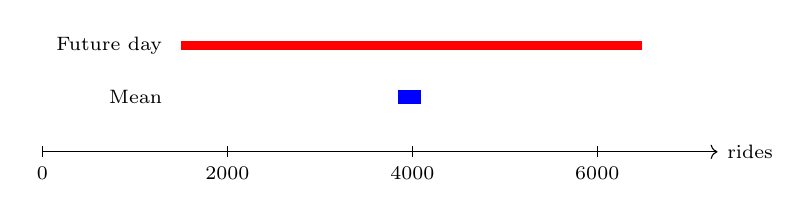
\begin{tikzpicture}[x=.00118cm,y=1cm]
\draw[->] (0,0)--(7300,0) node[right]{\scriptsize rides};
\foreach \x in {0,2000,4000,6000} {\draw (\x,.07)--(\x,-.07) node[below]{\scriptsize\x};}
\draw[line width=5pt,blue] (3843,.7)--(4095,.7);
\node[left] at (1400,.7) {\scriptsize Mean};
\draw[line width=3pt,red] (1500,1.35)--(6482,1.35);
\node[left] at (1400,1.35) {\scriptsize Future day};
\end{tikzpicture}

\par\medskip\textbf{Decision lesson:} narrow uncertainty around the average cannot justify a narrow reserve for a single day.
\end{frame}

\begin{frame}{From forecasts to operational risk}
A manager needs event probabilities, not just a point forecast:
\[\Prob(Y_{\mathrm{new}}>K\mid X=75,\dd)\]
where $K$ is the capacity that can be served.

\begin{itemize}
\item $K=5000$: probability that demand exceeds 5,000 rides.
\item $K=3000$: probability that demand falls below 3,000 rides.
\end{itemize}
\par\medskip
\textbf{With posterior predictive draws:}
\[\widehat{\Prob}(Y_{\mathrm{new}}>K\mid\dd)=\frac{\#\{Y_{\mathrm{new}}^{(s)}>K\}}{S}.\]
These probabilities directly support inventory and staffing decisions.
\end{frame}

\begin{frame}{Worked example: approximate tail risk}
For a hand calculation only, approximate the prediction by
\[Y_{\mathrm{new}}\mid75,\dd\ \dot\sim\ N(3968,1280^2).\]
Then, using a standard Normal table,
\[\Prob(Y_{\mathrm{new}}>5000)\approx 1-\Phi\!\left(\frac{5000-3968}{1280}\right)
=1-\Phi(0.806)\approx0.21.\]
\textbf{Interpretation:} roughly 21\% chance of demand exceeding 5,000 rides \emph{under this illustrative approximation}.
\par\medskip
\scriptsize The full posterior predictive interval, not this exact tail probability. For real analysis compute tail risk from \texttt{posterior\_predict()} draws rather than a Normal approximation.
\end{frame}

\begin{frame}{A capacity decision needs a loss model}
\textbf{Scenario (illustrative costs, not from the book):}
\begin{itemize}
\item \textbf{Standard capacity} (5,000 rides): no extra upfront cost, but a high-demand shortfall event creates a simplified \$4,000 loss.
\item \textbf{Expanded capacity}: costs an extra \$600 and is assumed to eliminate that shortfall loss for this example.
\end{itemize}
Define $H=\{Y_{\rm new}>5000\}$. The loss matrix is
\[\begin{array}{c|cc}
& H & H^c\\\hline
\text{Standard} &4000&0\\
\text{Expanded}&600&600
\end{array}\]
\scriptsize A real loss function would account for the \emph{size} of each shortfall, capacity limits, and other costs.
\end{frame}

\begin{frame}{Choose the action with lower expected loss}
Using the illustrative $\Prob(H\mid\dd)\approx0.21$:
\begin{align*}
\E[L(\text{Standard})\mid\dd]&=4000(0.21)+0(0.79)=\$840,\\
\E[L(\text{Expanded})\mid\dd]&=\$600.
\end{align*}
So \textbf{expanded capacity} has lower expected loss in this scenario.
\par\medskip\textbf{General threshold:} expand when
\[4000\Prob(H\mid\dd)>600\quad\Longleftrightarrow\quad \Prob(H\mid\dd)>0.15.\]
This separates a statistical estimate (risk probability) from a management preference (cost of mistakes).
\end{frame}

\begin{frame}{Sensitivity analysis: what would reverse the choice?}
\small
\begin{tabular}{c|c|c}
\toprule Assumed high-demand risk & Expected standard loss & Preferred action\\\midrule
10\% & \$400 & Standard\\
15\% & \$600 & Tie\\
21\% & \$840 & Expanded\\
30\% & \$1,200 & Expanded\\\bottomrule
\end{tabular}
\vspace{.4cm}
\begin{itemize}
\item Changing the event cost also changes the threshold.
\item Forecast uncertainty, data bias, and wrong model assumptions may change $\Prob(H)$.
\item A robust decision considers plausible alternatives, not just one model run.
\end{itemize}
\end{frame}

\begin{frame}{Decision risk is broader than residual noise}
\begin{enumerate}
\item \textbf{Parameter risk:} uncertain intercept, slope, and residual SD.
\item \textbf{Outcome risk:} random variation even if parameters were known.
\item \textbf{Model risk:} nonlinearity, heteroskedasticity, seasonality, autocorrelation, count boundaries.
\item \textbf{Decision risk:} wrong costs, missing operational constraints, or forecast error in $X$.
\end{enumerate}
\end{frame}

\begin{frame}{Sequential learning can change the decision}
The book re-fits after $30$, $60$, and $500$ observed days.
\begin{itemize}
\item Early winter days cover a narrow temperature range; slope estimates may be uncertain or misleading.
\item As data span more temperatures, the inferred relationship changes and tightens.
\item Revisit forecast risks and capacity decisions as new evidence arrives.
\end{itemize}
\par\medskip
\textbf{Warning:} having more observations is not always enough; \emph{coverage of decision-relevant conditions} matters.
\end{frame}

\begin{frame}{When prior information is weak}
\begin{itemize}
\item They can allow positive, flat, or negative slopes rather than asserting a strong prior increase.
\item Autoscaling adapts prior scale to data units; check the resulting prior with \texttt{prior\_summary()}.
\item Simulate prior predictive datasets and assess realistic magnitudes.
\end{itemize}
\par\medskip
\textbf{Decision impact:} a weak prior may produce wider predictive tails, especially with limited data. Compare choices across reasonable prior specifications.
\end{frame}

\begin{frame}[fragile]{R: predictive risk and decision rule}
\footnotesize
\begin{verbatim}
new_day <- data.frame(temp_feel = 75)
y_sim <- posterior_predict(bike_model,
                           newdata = new_day)
y_sim <- as.numeric(y_sim)

p_short <- mean(y_sim > 5000)
loss_standard <- 4000 * p_short
loss_expanded <- 600

c(p_short = p_short,
  loss_standard = loss_standard,
  loss_expanded = loss_expanded)
\end{verbatim}
\scriptsize Use the simulation output as the primary risk estimate. The earlier 21\% was only an approximate classroom calculation.
\end{frame}

\begin{frame}{Homework (part 1)}
\begin{itemize}
\item[] 9.10.1 Conceptual exercises
\begin{itemize}
\item Exercise 9.1
\item Exercise 9.2
\item Exercise 9.3
\item Exercise 9.4
\item Exercise 9.5
\end{itemize}
\item[] 9.10.2 Applied exercises
\begin{itemize}
\item Exercise 9.9
\item Exercise 9.10
\end{itemize}
\end{itemize}
\end{frame}

\begin{frame}{Homework (part 2)}
A manager can buy expanded capacity for \$600. The cost of failing to meet demand above 5,000 rides is \$4,000 (simplified event loss).
\begin{enumerate}
\item If $\Prob(Y_{\rm new}>5000\mid\dd)=0.12$, what action minimizes expected loss?
\item If the shortage cost rises to \$7,500, how does the threshold change?
\item What if your Normal predictive model assigns negative rides some probability?
\item Which additional predictor or diagnostic would most improve this decision?
\end{enumerate}
\par\medskip
\scriptsize \textbf{Answers:} (1) Standard: $\$480<\$600$. (2) Threshold $600/7500=0.08$, so expand at risk 0.12. (3) Check model adequacy and consider alternatives. (4) Reasonable answers include day-of-week and seasonality.
\end{frame}

\begin{frame}{Takeaways: model $\rightarrow$ uncertainty $\rightarrow$ decision}
\begin{enumerate}
\item Choose a data model and mean structure that reflect the substantive problem.
\item Use defensible priors, posterior simulation, and diagnostics.
\item For actions involving one future day, use the \emph{posterior predictive}, not a confidence interval for the mean.
\item Translate predictive draws into event probabilities and expected losses.
\item Stress-test the choice against prior sensitivity, model misspecification, and uncertain costs.
\end{enumerate}
\end{frame}
\end{document}